
\clearpage
\section{Customer Relationship Management}

Das CRM (Customer Relationship Management) ermöglicht Ihnen effizient Veranstaltungen (Anlässe, Präsentationen und Schulungen) zu koordinieren. Es unterstützt Sie bei der Einladung, dem Verwalten von Anmeldungen, Versenden von Erinnerungen und dem Erstellen von Teilnehmerlisten.

\vspace{\baselineskip}

Für Ihre Veranstaltung erstellen Sie über eine Webseite eine Einladung in Form eines Online-Flyers mit den wichtigsten Angaben zum Anlass, Eckdaten wie Termin, Zeit, Bemerkungen und Weiteres. Die Einladung, welche auf diese Einladungsseite verweist, versenden Sie aus dem CRM an eine gewünschte Personengruppe. Die Eingeladenen können über diese Webseite Ihre Anmeldung am Anlass durchführen (mittels Klick) oder falls notwendig zu Beginn oder später Ihre Entschuldigung einreichen. Sie als Organisator haben jederzeit den Überblick über die versendeten Einladungen und deren Status. Sie sehen sofort wie viele Personen sich bereits an- oder abgemeldet haben. \\

Schliesslich können Sie eine Teilnehmerliste exportieren und können auf diese Weise das Resultat Ihrer Einladung auswerten oder weiterreichen.

\vspace{\baselineskip}

Das CRM ist in zwei Teile gegliedert: 
\begin{itemize}
\item
\textbf{Veranstaltungstypen:} Hier legen Sie die verschiedenen Arten von Veranstaltungen fest (bspw. Jahresrückblick, Neuheiten-Präsentation etc.)
\item
\textbf{Veranstaltungen:} Unter diesem Menüpunkt werden die konkreten Veranstaltungen geplant. Nach dem Anlegen einer Veranstaltung haben Sie die Möglichkeit, die Einladungswebseite (Online-Flyer) zu gestalten.
\end{itemize}

\pagebreak
\subsection{Veranstaltungstypen}

\begin{wrapfigure}[7]{l}{6.5cm}   % [x] Wie manche Zeile soll sich um die Grafik "brechen"
  \vspace{-35pt}      % Grundwert war 20; mit 30 schön oben beim Text ausgerichtet
  \begin{center}
    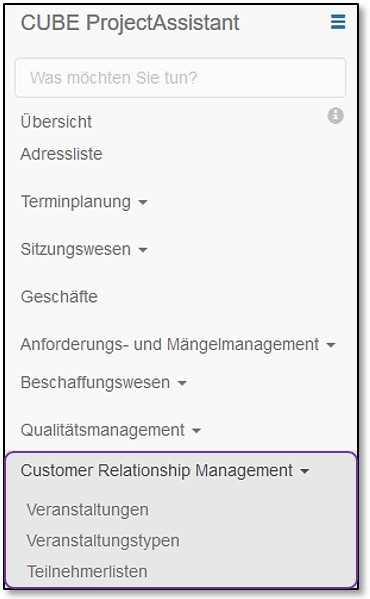
\includegraphics[width=1\linewidth]{../chapters/10_CRM/pictures/10-1-1_Menu_CRM.jpg}
  \end{center}
  \vspace{-20pt}
  \caption{Das CRM Menü}
  \vspace{-10pt}
\end{wrapfigure}

\textbf{Übersicht:} Klicken Sie im Menü links auf 'Customer Relationship Management' und den Unterpunkt Veranstaltungstypen.\\


\textbf{Hinweis:} Bevor Sie mit dem Erstellen einer Veranstaltung beginnen, erfassen Sie den oder die gewünschten Veranstaltungstyp/en. 

\vspace{8cm}

Die Übersicht der Veranstaltungstypen öffnet sich:

\begin{figure}[H]
\center{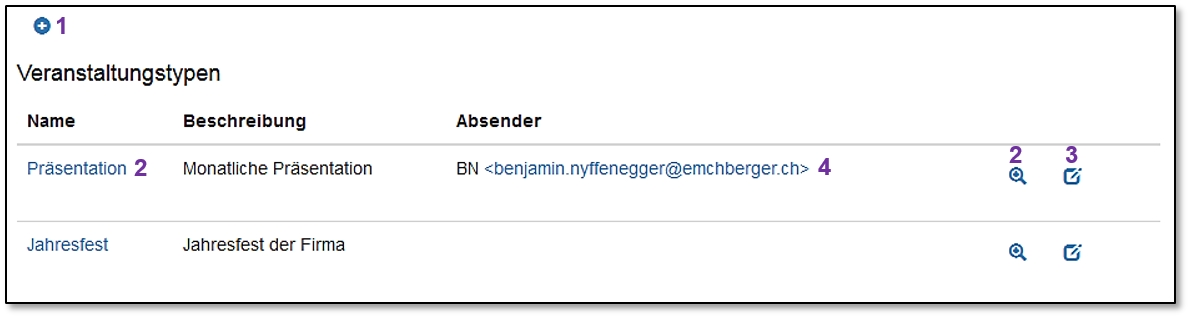
\includegraphics[width=1\linewidth]{../chapters/10_CRM/pictures/10-1_VeranstTyp_Uebersicht.jpg}}
\caption{Übersicht Veranstaltungstypen}
% \label{fig:speciation}
\end{figure}

Sie sehen alle erfassten Veranstaltungstypen. Mit Klick auf das Plussymbol 
\includegraphics[height=12pt]{/Icons/Plussymbol.jpg} \col{(1)} können Sie einen neuen Veranstaltungstyp erstellen. Mit Klick auf den entsprechenden Veranstaltungstyp \col{(2)} oder auf das Lupensymbol 
\includegraphics[height=12pt]{/Icons/Lupe.jpg} \col{(2)} können Sie die Details eines Veranstaltungstypen betrachten. Um einen Eintrag zu bearbeiten, klicken Sie auf das Bearbeiten-Symbol 
\includegraphics[height=12pt]{/Icons/Bearbeiten.jpg} \col{(3)}. Wurde eine Absender-Emailadresse hinterlegt, können Sie mit Klick auf diese \col{(4)} eine Email versenden. Wählen Sie das gewünschte Emailprogramm aus.

\subsubsection{Neue Veranstaltungstypen anlegen}

\begin{figure}[H]
\center{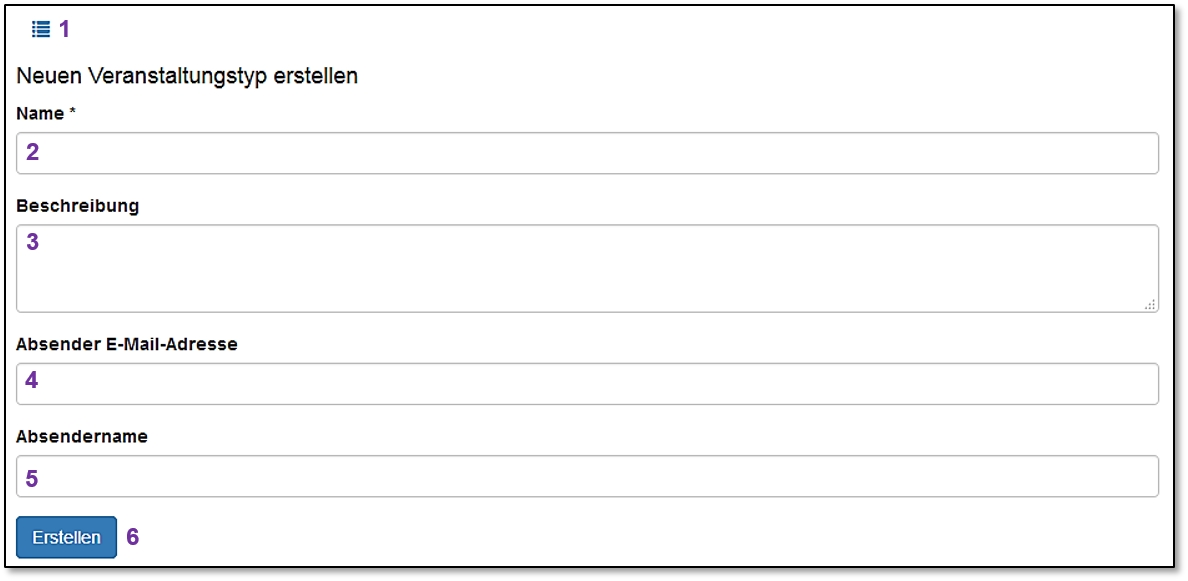
\includegraphics[width=1\linewidth]{../chapters/10_CRM/pictures/10-1_VeranstTyp_erstellen.jpg}}
\caption{Neue Veranstaltungstypen erstellen}
% \label{fig:speciation}
\end{figure}

Mit Klick auf das Listensymbol 
\includegraphics[height=12pt]{/Icons/Listensymbol_zurueck.jpg} \col{(1)} kehren Sie jederzeit auf die Übersicht zurück.\\
Geben Sie einen aussagekräftigen Namen \col{(2)} für den gewünschten Veranstaltungstyp ein (Dies ist ein Pflichtfeld und muss als einziges ausgefüllt werden.) Unter 'Beschreibung' \col {(3)} können Sie den Veranstaltungstyp präziser beschreiben. Sie haben die Möglichkeit eine Absender-Emailadresse \col{(4)} und einen Absendernamen \col{(5)} zu hinterlegen. Wird eine Emailadresse eingetragen, können Sie in der Übersicht mit Klick auf die Emailadresse direkt eine Email versenden. Nach den Eingaben schliessen Sie den Vorgang mit 'Erstellen' \col{(6)} ab.

\subsubsection{Bestehende Veranstaltungstypen betrachten und bearbeiten}

\begin{wrapfigure}[12]{l}{6.5cm}   % [x] Wie manche Zeile soll sich um die Grafik "brechen"
  \vspace{-35pt}      % Grundwert war 20; mit 30 schön oben beim Text ausgerichtet
  \begin{center}
    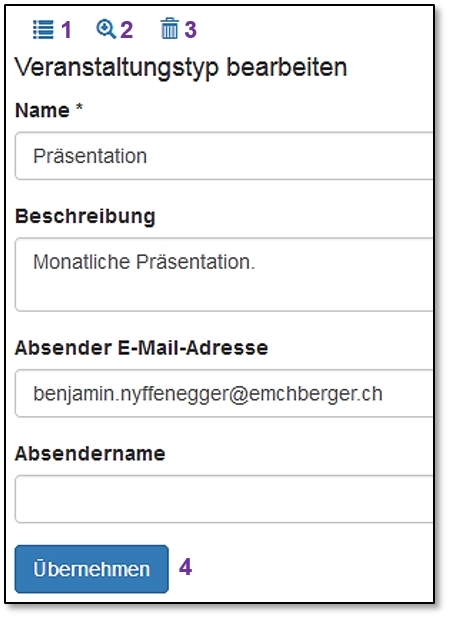
\includegraphics[width=1\linewidth]{../chapters/10_CRM/pictures/10-1-2_Veranstaltungstyp_bearbeiten.jpg}
  \end{center}
  \vspace{-20pt}
 % \caption{Veranstaltungstyp bearbeiten}
  \vspace{-10pt}
\end{wrapfigure}

Klicken Sie in der Übersicht der Veranstaltungstypen auf das Bearbeiten-Symbol 
\includegraphics[height=12pt]{/Icons/Bearbeiten.jpg}, um einen bereits erstellen Eintrag zu ändern. Die Maske mit den ausgefüllten Feldern wird geöffnet. Schliessen Sie diesen Vorgang mit Klick auf 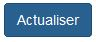
\includegraphics[height=12pt]{/Icons/B_Uebernehmen.jpg} \col{(4)} ab. Die Maske wird nicht automatisch geschlossen. Mit Klick auf das Listensymbol 
\includegraphics[height=12pt]{/Icons/Listensymbol_zurueck.jpg} \col{(1)} kehren Sie zur Übersicht zurück. Sie können mittels dem Lupensymbol 
\includegraphics[height=12pt]{/Icons/Lupe.jpg} \col{(2)} den Eintrag betrachten. Im Bearbeitungsmodus haben Sie zudem die Möglichkeit, mittels Klick auf das Mülltonnensymbol 
\includegraphics[height=12pt]{/Icons/Muelltonne.jpg} \col{(3)} einen Eintrag zu löschen.

\vspace{\baselineskip}

\subsection{Veranstaltungen}

\textbf{Übersicht}

\begin{figure}[H]
\center{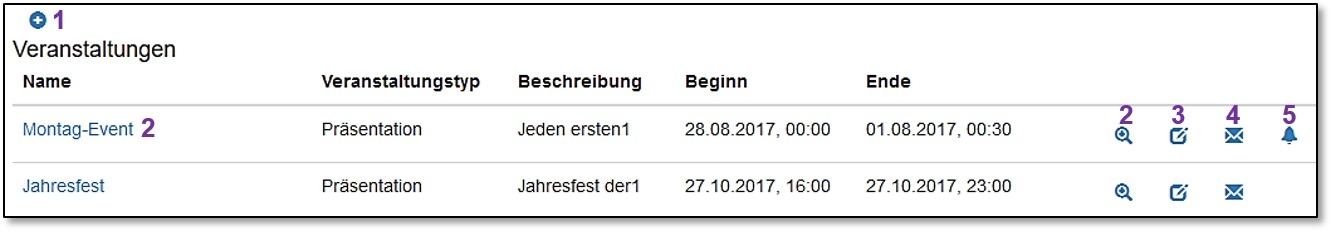
\includegraphics[width=1\linewidth]{../chapters/10_CRM/pictures/10-2_Veranstaltungen_Uebersicht.jpg}}
\caption{Übersicht Veranstaltungen}
% \label{fig:speciation}
\end{figure}

Text x

\subsubsection{Neue Veranstaltungen anlegen}

Text x

\subsubsection{Einladungsseite gestalten (Online-Flyer)}

Text x

\subsubsection{Teilnehmer verwalten}

inkl. Export
inkl. neue Person erfassen (Adressliste)
hinzufügen, löschen, Status ändern, 


\subsubsection{Einladungen versenden}

inkl. Emailvorlage bearbeiten

\subsubsection{Bestehende Veranstaltungen betrachten und bearbeiten}

Veranstaltung löschen
Text x

